% !TeX root = ../main.tex
\clearpage
\setlength{\parskip}{0pt}\chapter{Thermally bi-directionally tunable (TBDT) AWG} \label{chap:3}
    \lipsum

\section{Simulation for passive design} \label{sec:3.1}
    \lipsum

\section{Simulation for active design} \label{sec:3.2}
    \lipsum

\section{Measurement results} \label{sec:3.3}
    \lipsum
    \begin{figure}[!b]
		% \includegraphics[scale = 1.25]{/TBDTAWG/TBDTAWG_Fig7_revised_300dpi.pdf}
        \noindent\makebox[\textwidth]{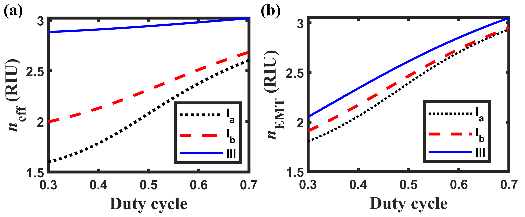
\includegraphics[width=\textwidth]{Fig_sample.pdf}}
		\centering
		\caption{\label{fig:tbdtawgmeadneff_vb}Effective index differences (left y axis) of adjacent AWs and wavelength shifts (right
                                            y axis) of filtering response in terms of electrical voltages at four output Channels 1.27, 1.29,
                                            1.31, and 1.33 \textmu m for \textbf{(a--d)} red-shift tuning and \textbf{(e--h)} blue-shift tuning, 
                                            where the solid line and squared red marker represent the simulated results from Fig.~\ref{fig:tbdtawgsimdneff} 
                                            and the measured data from Fig.~\ref{fig:tbdtawgmeaspec}, respectively.}
	\end{figure}
    \lipsum
    \begin{table}[!b]
		\caption{\label{tab:ttawgcompare}
		Thermal-tuning performance comparison of thermally tunable AWGs in the literature.}
		\centering
		% \begin{ruledtabular}
		% \begin{tabular}{|P{0.6in}|P{0.45in}|P{0.45in}|P{0.45in}|P{0.45in}|P{0.45in}|}	\hline
        %.......................................... For dissertation, total width = 4.75 inches ................................................
        %.......................................... For IEEE journal (two-column), total width = 3.5 inches ..........................
        % \begin{tabular}{|M{0.6in}|M{0.27in}|M{0.25in}|M{0.3in}|M{0.2in}|M{0.3in}|M{0.4in}|}	\hline % well fit for IEEE
		\begin{tabular}{|M{0.76in}|M{0.61in}|M{0.68in}|M{0.76in}|M{0.5in}|M{0.55in}|M{0.89in}|}	\hline % well fit for IEEE
            % \rowcolor{lightgray}\makecell{Literature\textbackslash\\Performance} & 
            \rowcolor{lightgray}\makecell{Literature} & 
            \textcolor{black}{Tuning efficiency} & 
            \textcolor{black}{Tuning direction} & 
            \textcolor{black}{Applied voltage} & 
            \textcolor{black}{Tuning range} & 
            \textcolor{black}{Platform} & 
            \textcolor{black}{TO coefficient} \\ \hline
            
            2020~\cite{TTAWG-p1} & \makecell{6.4\\nm/W} & Red & 40~V for 2.3-nm shift & 
                    2.5~nm & Silicon & 1.68$\cdot 10^{-4}$~/K \\ \hline
            2015~\cite{TTAWG-p3} & \makecell{$\sim$3.97\\nm/W} & Red & 40~V for 5-nm shift & 
                    5~nm & Silicon; SiO$_2$ & \makecell{1.84$\cdot 10^{-4}$~/K;\\1$\cdot 10^{-5}$~/K}\\ \hline
            1999~\cite{TTAWG-n1} & -- & Blue & -- & 
                    9~nm & Polymer & \symbol{"2212}1.6$\cdot 10^{-4}$~/K \\ \hline
            2006~\cite{TTAWG-n2} & -- & Blue & -- & 
                    6.6~nm & Polymer/Si & \symbol{"2212}1.16$\cdot 10^{-4}$~/K \\ \hline
            1999~\cite{TBDTAWG} & \makecell{$\pm2$\\nm/W} & Bi-directional & -- & 
                    6~nm & SiO$_2$--Si & positive \\ \hline
            \textbf{Proposed Device} & \makecell{\textbf{$\pm$30.5}\\nm/W} & \textbf{Bi-directional} & 
                    \textbf{2.5~V for $\pm$8-nm shift} & 
                    \textbf{$\ge\,$8~nm} & Silicon & 1.68$\cdot10^{-4}$~/K \\ \hline
		\end{tabular}
		% \end{ruledtabular}
        % \begin{flushleft}
			% \SP{a} 1-dB bandwidth measured from the transmission peak\\	
			% \SP{b} Available bandwidth (ABW) for channel XT below \symbol{"2212}25~dB\\	
			% \SP{c} Echelle grating; \SP{d} Multi-mode interferometer; \SP{e} Waveguide Bragg grating. \\
		% \end{flushleft}
	\end{table}
    an index change $\upDelta n_\text{eff}$ of $\pm$0.0114 and a shift $\upDelta \lambda$ of $\pm$8~nm 
    are obtained from the measured results,
    indicating a linear bi-directional shift-to-power ratio of $\pm$30.5~nm/W with a wide tuning range
    of 8~nm. The difference of absolute values of linear ratios between simulation (36.07~nm/W)
    and measurement (30.5~nm/W) might come from the power loss in the electrical metal traces or
    from a deviated thickness and/or sheet resistance of the fabricated heating wire. 
    A performance comparison is given in Table~\ref{tab:ttawgcompare}, 
    showing a better thermal-tuning efficiency with bi-directional tuning functions for the proposed device.
    
\section{Discussion} \label{sec:3.4}
    \lipsum

\section{Summary} \label{sec:3.5}
    \lipsum
